\documentclass[12pt]{article}

\usepackage[margin=1in]{geometry}
\usepackage[T1]{fontenc}
\usepackage{lmodern}
\usepackage{graphicx}
\usepackage{booktabs}
\usepackage{caption}
\usepackage{float}
\usepackage{placeins}
\usepackage[hidelinks]{hyperref}

\graphicspath{{../figures/}{figures/}}
\captionsetup{font=small, labelfont=bf}
\setlength{\parskip}{0.25em}
\setlength{\textfloatsep}{12pt plus 2pt minus 4pt}

\begin{document}

% ---------------------------------------------------------------------------
% Title page (not counted in the 8 pages)
% ---------------------------------------------------------------------------
\pagenumbering{roman}
\begin{titlepage}
\centering
\vspace*{3cm}
{\LARGE\bfseries Fewer Fires, Bigger Burns\par}
\vspace{0.4cm}
{\Large Where Is Canada's Burned Area Coming From?\par}
\vspace{1.5cm}
{\large COMP 6934 -- Final Project Report\par}
{\large Team 9\par}
\vspace{2cm}
\begin{tabular}{ll}
\toprule
\textbf{Name} & \textbf{Student ID} \\
\midrule
Amar Preet Singh    & 202680417 \\
Samridh Barthaval   & 202582280 \\
Prakash Periyasamy  & 202681309 \\
\bottomrule
\end{tabular}
\vfill
{\large Memorial University of Newfoundland\par}
{\large Fall 2026\par}
\end{titlepage}
\pagenumbering{arabic}

% ---------------------------------------------------------------------------
\section{Introduction}

Our data is the fire point file of the \emph{Canadian National Fire Database}
(NFDB), published by Natural Resources Canada under the Open Government
Licence -- Canada~\cite{nfdb}. We use the version dated 11~August~2026. Each row
is one wildfire reported by a province, a territory or Parks Canada. The file
has 448,618 fires going back to the 1940s and 24 columns. For every fire we
know where it started (latitude and longitude), which agency reported it, the
date it was reported, its final size in hectares and its cause, which is
coded as human (H), natural/lightning (N) or unknown (U). The file also has an
``out'' date, a fire type and a few agency-specific columns, but these are
filled in very unevenly.

We picked this dataset because of the last few fire seasons. In 2023 Canada
had its worst season on record: the fires in this file add up to 17.6 million
hectares, more than twice the previous record from 1989. 2025 was the second
worst year at 8.7 million hectares. Wildfires matter for forestry, for
people's health through smoke, for emergency planning, and especially for
Indigenous and northern communities that get evacuated. As students living in
Canada we hear about smoke and evacuations every summer, and we wanted to see
what the data says about these record years.

\section{Questions}

The headline numbers seem to go in opposite directions: Canada reports fewer
fires than it used to, but more land is burning. Our main question is
therefore:

\begin{quote}
\emph{Where is Canada's burned area coming from?}
\end{quote}

The NFDB has no weather or climate information, so we cannot say \emph{why}
fires are getting bigger. What we can do is describe which fires make up the
burned area, in terms of their size, cause, location and start date. We split
the main question into five smaller ones:

\begin{enumerate}\setlength{\itemsep}{0pt}
  \item How have the number of fires and the area burned changed since 1980,
        and how unusual were 2023 and 2025? Is the drop in fire numbers real,
        or a change in reporting?
  \item Does most of the burned area come from a few very big fires?
  \item How do human-caused and lightning-caused fires differ in number and
        in area burned?
  \item Where do the big fires happen?
  \item When in the year do fires start, and did 2023 and 2025 start earlier
        than usual?
\end{enumerate}

\section{Data preparation}

We keep the years 1980 to 2025. Before that the record is not complete:
Ontario and Quebec only start reporting in the mid-1970s, and Saskatchewan in
1980. All cleaning is done in one Python script
(\texttt{make\_figures.py}), which also makes every figure in this report.
Table~\ref{tab:cleaning} lists what we did with each problem we found.

\begin{table}[ht]
\centering
\small
\begin{tabular}{p{5.4cm}p{9.4cm}}
\toprule
\textbf{Problem} & \textbf{What we did} \\
\midrule
Years before 1980, or $-999$ & Removed (108,439 rows). 340,179 fires remain. \\
Prescribed burns & Removed (438). They are planned fires, not wildfires.
  Agencies flag them in different columns, so we checked all of them. \\
Exact repeated rows & Removed 1,201 rows that have the same agency, date,
  location, size and cause (82,900~ha in total). The fire ID alone is not
  unique, because some agencies reuse IDs for different fires. \\
Positive longitudes & 83 fires (mostly Newfoundland and Labrador, 2022--25)
  are missing the minus sign. We flipped the sign. \\
Impossible locations & 117 fires are still outside Canada (e.g.\ at 0,~0).
  Kept in all totals, left off the map. \\
Fires of 0~ha & 29,525 fires. Kept, since they are real reports; only left
  out of the log-scale histogram. \\
Unknown start month (0) & 3,459 fires, mostly Manitoba 2000--2003. Left out of
  the month heatmap only. \\
No ``out'' date & 37.8\% of fires. We do not use this column. \\
\bottomrule
\end{tabular}
\caption{Data problems and how we handled them. After cleaning, 338,540 fires
from 1980--2025 remain.}
\label{tab:cleaning}
\end{table}

% ---------------------------------------------------------------------------
\section{Results}

\subsection{Fewer fires, but more area burned}

\begin{figure}[t]
\centering
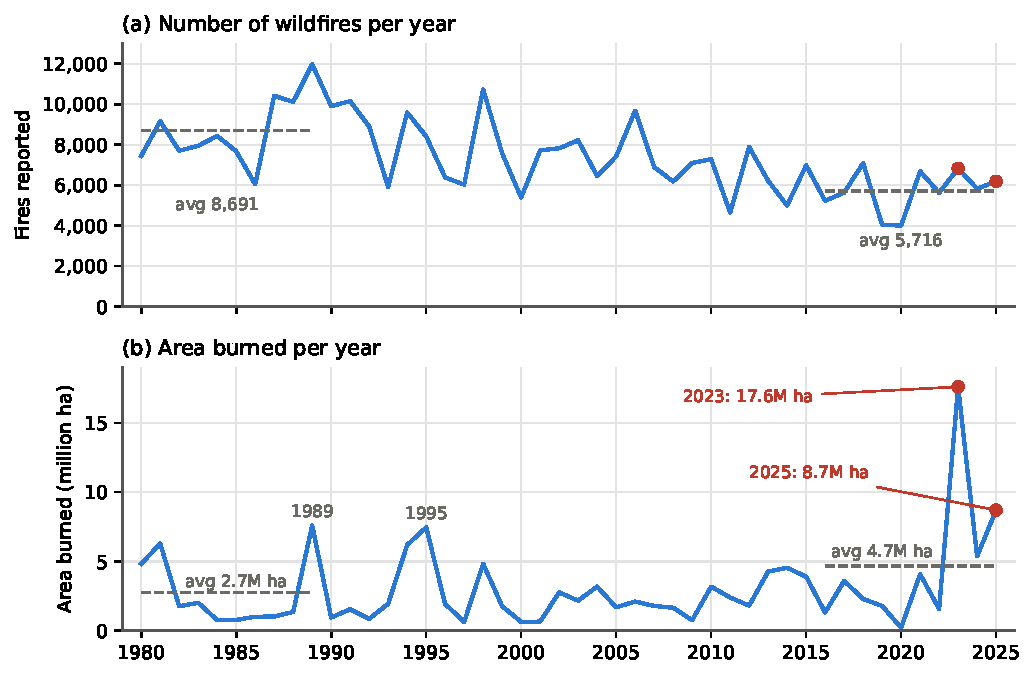
\includegraphics[width=0.92\textwidth]{fig1_yearly_trend.pdf}
\caption{Number of wildfires (a) and area burned (b) per year, 1980--2025.
Dashed lines are the averages for 1980--89 and 2016--25. Fires went down by
about a third while the average area burned went up by about 70\%, and 2023
(17.6~Mha) is far above every other year.}
\label{fig:yearly}
\end{figure}

Figure~\ref{fig:yearly} shows the starting point of our project. In the 1980s
agencies reported on average 8,691 fires a year; in the last ten years
(2016--25) the average is 5,716, a drop of 34\%. Over the same periods the
average area burned went up from 2.7 to 4.7 million hectares (Mha) a year.
The area line is also much more ``spiky'' than the count line. A typical year
burns about 1.9~Mha (the median), and a few years stand far above it: 1989,
1995, 2025 and above all 2023. With 17.6~Mha, 2023 burned about nine times a
typical year and 2.3 times the old record of 1989. 2025 is the second largest
year at 8.7~Mha. What stands out is that both of these years had an ordinary
number of fires (6,837 and 6,215). The record area did not come from more
fires.

\begin{figure}[t]
\centering
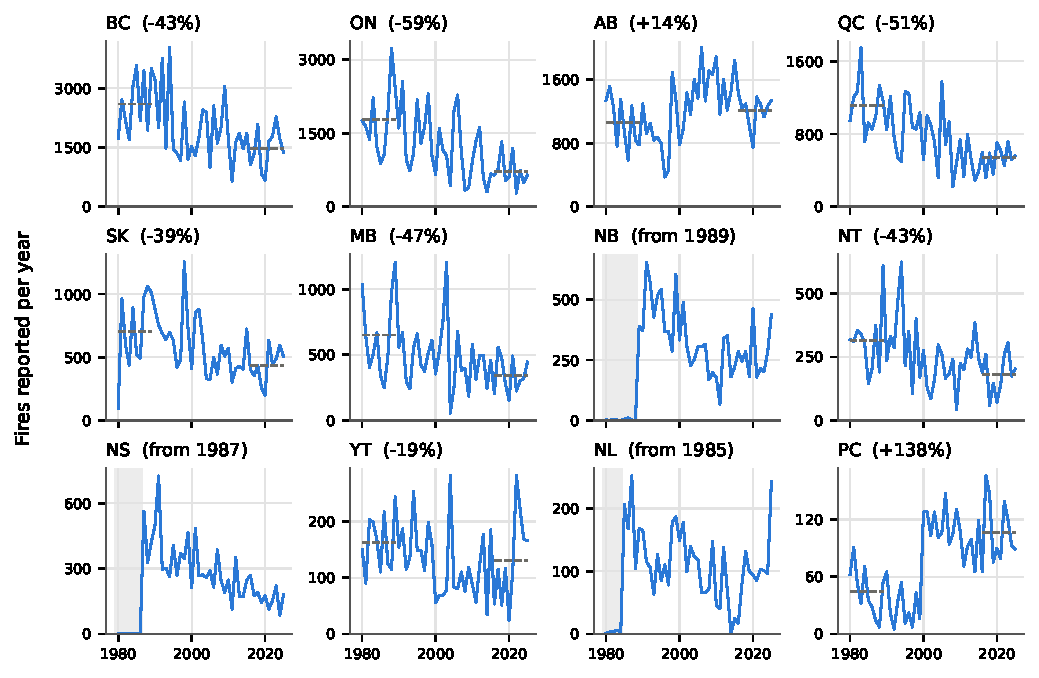
\includegraphics[width=0.9\textwidth]{fig2_agencies.pdf}
\caption{Fires reported per year by each agency (each panel has its own
y-axis; PEI is left out, it has only 55 fires). The percentage is the change
between the 1980--89 and 2016--25 averages (dashed). Grey areas mark years
before NB, NS and NL sent full records. The drop in figure~\ref{fig:yearly}a
shows up in almost every agency, so it is not caused by one agency changing
how it reports.}
\label{fig:agencies}
\end{figure}

Before we trust the drop in fire numbers, we have to check that it is not a
reporting effect, for example one agency that stopped sending small fires.
Figure~\ref{fig:agencies} splits the counts by agency. Nine agencies have full
records since 1980, and seven of them report fewer fires now than in the
1980s: Ontario ($-59\%$), Quebec ($-51\%$), Manitoba ($-47\%$), British
Columbia ($-43\%$), the Northwest Territories ($-43\%$), Saskatchewan ($-39\%$)
and Yukon ($-19\%$). Only Alberta ($+14\%$) and Parks Canada, which is small
and whose counts jump around 2000, go up. Taken together, these nine agencies
went from 8,427 to 5,157 fires a year ($-39\%$), slightly more than the
national drop. New Brunswick, Nova Scotia and Newfoundland and Labrador only
send full records from the late 1980s, so they push the national total
\emph{up} rather than down. Since the decline is spread across almost every
agency, we treat it as real. We still cannot rule out that some agencies
became stricter about which small fires they record, but there is no single
break that would point to that.

\subsection{A few very large fires make up almost all of the area}

\begin{figure}[t]
\centering
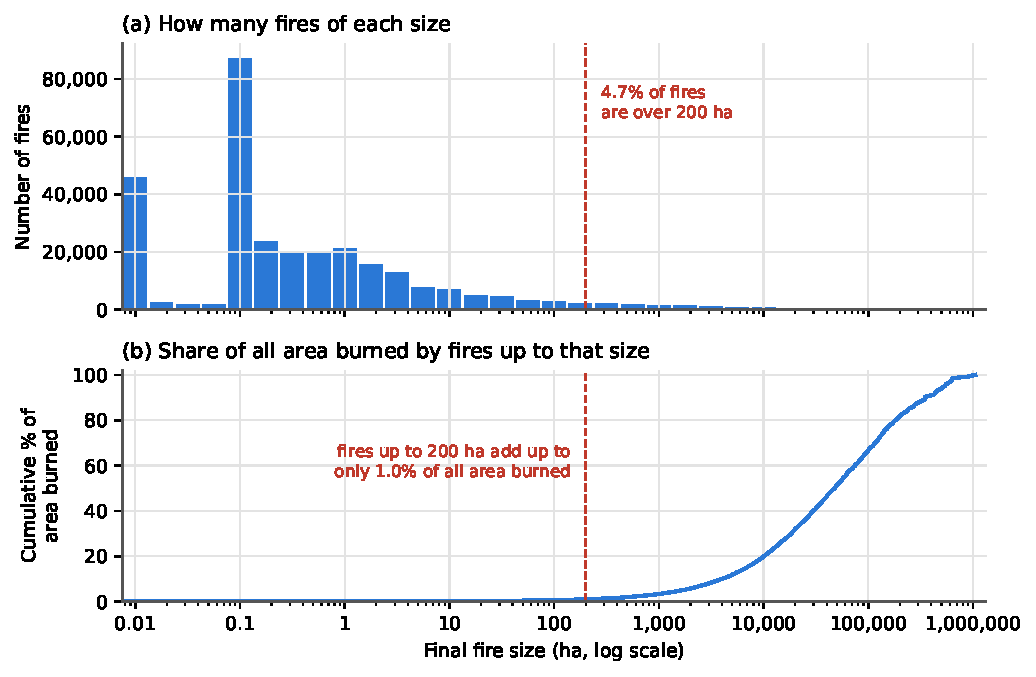
\includegraphics[width=0.9\textwidth]{fig3_size_distribution.pdf}
\caption{(a) Histogram of final fire size on a log scale (fires of 0~ha left
out). The spikes at 0.01 and 0.1~ha are sizes rounded by the agencies.
(b) Share of all area burned 1980--2025 that comes from fires up to a given
size. Fires larger than 200~ha are 4.7\% of all fires but 99\% of the area,
so the burned area is decided by the few very large fires.}
\label{fig:sizes}
\end{figure}

Figure~\ref{fig:sizes}a shows how many fires there are of each size. Most fires
are tiny: 71.5\% end below one hectare, and the most common recorded size is
0.1~ha. The right tail is long, with fires up to 1.05 million hectares.
Figure~\ref{fig:sizes}b uses the same x-axis to show the running total of area
burned. The curve stays flat at zero across all the small fires and only
starts to rise after a few hundred hectares. The 15,914 fires above 200~ha are only
4.7\% of all fires, but they burned 99.0\% of the area. Going further, the
2,613 fires of at least 10,000~ha (0.8\% of fires) account for 80.2\% of all
area burned.

This also explains figure~\ref{fig:yearly}. While the total number of fires
fell, the number of fires above 200~ha went \emph{up}, from 334 a year in the
1980s to 437 a year in 2016--25 ($+31\%$). 2023 had 953 such fires; the
previous highest was 751 in 1989. In 2023, 91\% of the area burned came from
fires of 10,000~ha or more. So the answer to the second question is clearly
yes: Canada's burned area is the area of its few very large fires, and the
small fires, even though they are most of the work for fire crews, hardly
change the total.

\subsection{Lightning fires are half the fires but almost all the area}

\begin{figure}[t]
\centering
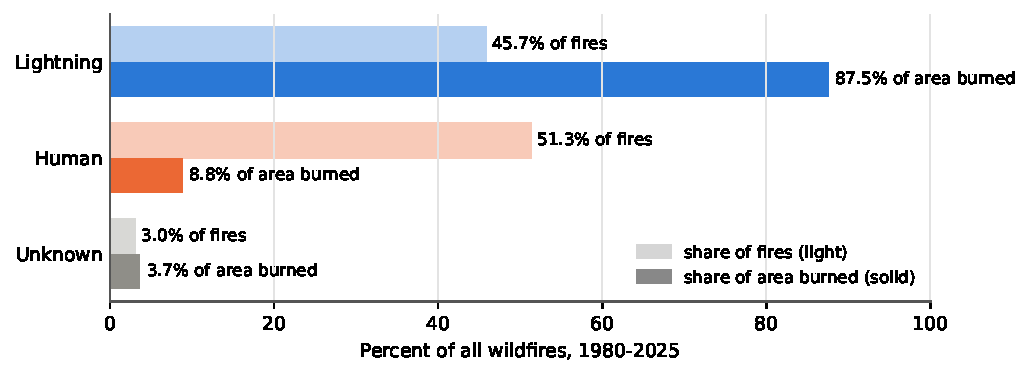
\includegraphics[width=0.85\textwidth]{fig4_cause_shares.pdf}
\caption{Share of all fires (light bars) and share of all area burned (solid
bars) for each cause, 1980--2025. Humans start slightly more than half of the
fires but these burn under 9\% of the area, while lightning fires burn
87.5\%.}
\label{fig:cause}
\end{figure}

Figure~\ref{fig:cause} compares the two main causes. People start 51.3\% of
all fires, a little more than lightning (45.7\%), but human-caused fires burn
only 8.8\% of the area. Lightning fires burn 87.5\%. The typical fire is
small for both causes (median 0.1~ha for human and 0.2~ha for lightning), so
the difference is all in the tail: 83\% of the fires above 200~ha were
started by lightning. In 2023 the lightning share of the area was even higher,
92\%. A likely reason, which we cannot test with this data, is that human
fires start close to roads and towns where they are seen early and attacked
quickly, while lightning fires often start in remote forest where they can
grow for days. The next figure supports the location part of this
explanation.

\subsection{The big fires are in the northern boreal forest}

\begin{figure}[t]
\centering
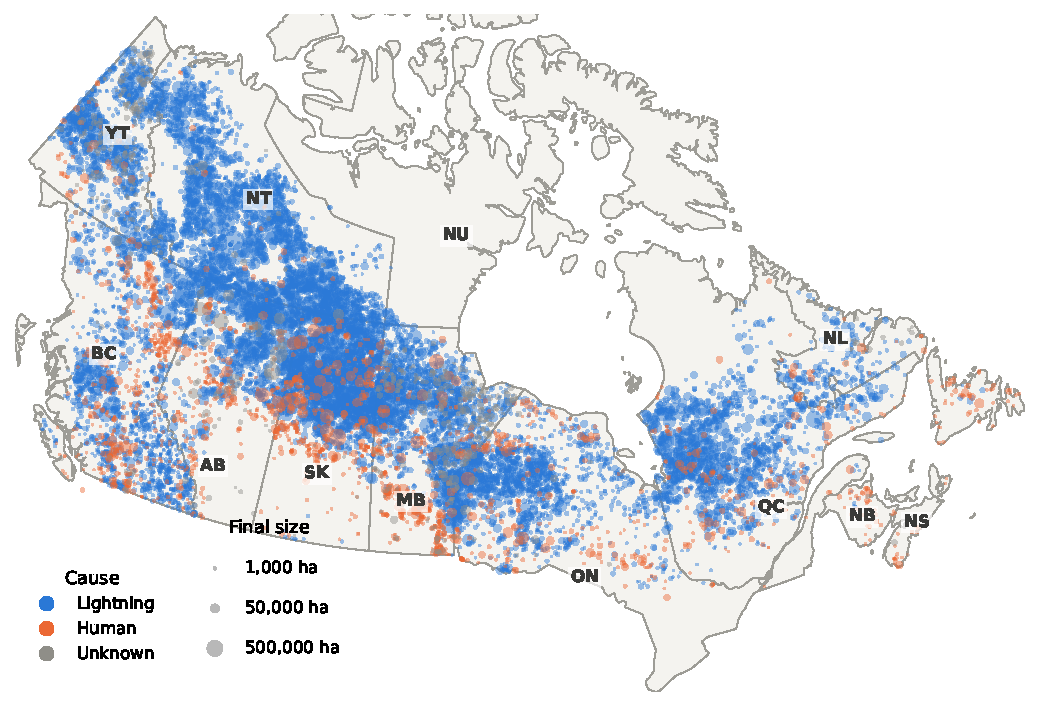
\includegraphics[width=0.88\textwidth]{fig5_big_fires_map.pdf}
\caption{Start locations of all fires larger than 200~ha, 1980--2025. Dot area
is proportional to final fire size and colour shows the cause. Large fires form
a band through the northern boreal forest from Yukon to Quebec, mostly started
by lightning; human-caused large fires sit along the southern edge of that
band, close to where people live.}
\label{fig:map}
\end{figure}

Figure~\ref{fig:map} maps the 15,914 fires above 200~ha (province outlines
from Natural Earth~\cite{ne}). They are not spread
evenly. Most of them form a wide band through the boreal forest: from Yukon
and the Northwest Territories, across northern Alberta, Saskatchewan and
Manitoba, into northern Ontario and Quebec. 68.8\% of their area lies north of
55\textdegree N, where few people live. The agencies with the most large-fire
area are the Northwest Territories (22\%) and Saskatchewan (19.5\%), followed
by Manitoba, Quebec, Alberta and British Columbia (8--12\% each). Ontario and
the Atlantic provinces have relatively few large fires, despite Ontario's high
fire count in figure~\ref{fig:agencies}. The orange dots (human cause) cluster
along the southern edge of the forest, near farmland, roads and towns in
central Alberta, Saskatchewan and Manitoba and in southern BC; 58\% of the
large human-caused fire area is south of 55\textdegree N. This matches the
idea from the previous section: the largest fires start where nobody is
around to stop them early.

\subsection{2023 and 2025 started early}

\begin{figure}[t]
\centering
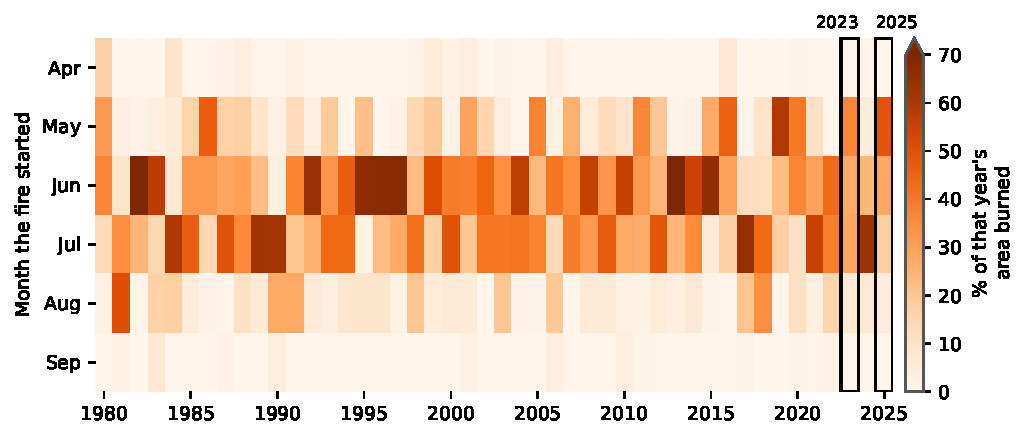
\includegraphics[width=0.95\textwidth]{fig6_month_heatmap.pdf}
\caption{Heatmap of how each year's area burned splits by the month the fires
started (each column sums to about 100\%; fires starting October to March
make up only 0.5\% of all area and are left out). In most years the area comes
from fires that start in June and July. In 2023 and 2025 (boxed) a much larger
share came from fires that started in May.}
\label{fig:heatmap}
\end{figure}

Figure~\ref{fig:heatmap} looks at the timing of the season. Each column is one
year, and the colour shows what share of that year's area came from fires
starting in each month. The darkest cells in most years are in June and July:
these are the months of the lightning season. In a typical year (the median),
only 15\% of the area comes from fires that started by the end of May. In
2023 this share was 37\% and in 2025 it was 49\%. In absolute terms, fires
that started in May 2023 burned 6.5~Mha, more than the whole of any other year
in the record except 1989, 1995 and 2025. In May 2025 it was 4.3~Mha, while a
typical May adds only about 0.2~Mha.

The heatmap also shows that an early start alone does not make a record year.
In 1980, 2016 and 2019 about half of the area also came from fires that
started by the end of May, but these years burned only 1.3 to 4.8~Mha in
total. What made 2023 different is that the early fires came on top of a very
active June and July: fires starting in June and July 2023 burned 4.8 and
5.0~Mha, each of these alone more than most full years. So 2023 had a season
that started early \emph{and} stayed active.

\FloatBarrier
% ---------------------------------------------------------------------------
\section{Conclusions}

We started with an apparent contradiction: fewer fires, but more area burned.
Our figures resolve it.

\begin{itemize}\setlength{\itemsep}{0pt}
  \item \textbf{The drop in fire numbers looks real.} Fires fell by about a
        third since the 1980s, in seven of the nine agencies with complete
        records (figures~\ref{fig:yearly} and~\ref{fig:agencies}).
  \item \textbf{The burned area comes from very few fires.} Fires over 200~ha
        are under 5\% of fires but 99\% of the area, and their number went
        up by 31\% while the total went down (figure~\ref{fig:sizes}). This
        is why the two lines in figure~\ref{fig:yearly} move apart.
  \item \textbf{Those fires are mostly lightning fires in the north.}
        Lightning starts under half of the fires but burns 87.5\% of the area
        (figure~\ref{fig:cause}), mostly north of 55\textdegree N
        (figure~\ref{fig:map}).
  \item \textbf{Record years start early and stay active.} 2023 and 2025 got
        a much bigger share of their area from May fires, and in 2023 June
        and July were also very large (figure~\ref{fig:heatmap}).
\end{itemize}

So, to answer our question: Canada's burned area comes from a small number of
very large, mostly lightning-caused fires in the remote northern forest, and
in the worst years from fires that started unusually early in the season.
Human-caused fires are more numerous, but they are smaller and closer to
people, so they add little to the total.

\textbf{Limitations.} The NFDB has no weather, fuel or fire-suppression data,
so our results describe the burned area but cannot explain the change. The
data are points: each fire's whole area is placed at its start location, which
is fine for large-scale patterns but not for exact fire footprints. Agencies
also differ in how they record size, cause and dates, and small fires are
often rounded to 0.1~ha. Joining the NFDB with fire-weather data, or using the
NFDB fire polygons, would be good next steps.

\textbf{Code.} All figures and numbers in this report are produced by
\texttt{make\_figures.py} from the 11~August~2026 copy of the data.

\textbf{Contributions.} All three team members contributed equally to this
project.

% ---------------------------------------------------------------------------
\begin{thebibliography}{9}\setlength{\itemsep}{0pt}
\small\raggedright
\bibitem{nfdb}
Canadian Forest Service. \emph{Canadian National Fire Database -- Agency Fire
Data}, fire point file, version 20260811. Natural Resources Canada, Canadian
Forest Service, Northern Forestry Centre, Edmonton, Alberta.
\url{https://cwfis.cfs.nrcan.gc.ca/ha/nfdb}

\bibitem{ne}
Natural Earth. \emph{Admin 1 -- States, Provinces}, 1:50m, version 5.1.1.
\url{https://www.naturalearthdata.com}
\end{thebibliography}

\end{document}
